\chapter{Implementation}\label{ch:implementation}
I det kommende afsnit, er løsningen blevet implementeret. Nu med planlægningen af kode (Analyse og design) er det muligt, at gå igang med næste aktivtitet under Unified Procces, implementation\cite{UnifiedProcess}. 

Koden er skrevet ud fra designklassediagrammet \ref{fig:designclassdiagram}, og benytter sig af de designmønstre som er vist i designklassediagrammet. Udover det er der også udviklet en GUI ud fra kravene oplyst i \ref{sec:mockup}. Koden er skrevet i Java. 
De vigtigste metoder og designmønstre vil blive demonstreret, herunder regression, parallelitet, singleton mønstret og database queries.

\section{Regression}
En måde at beregne den optimale bestillingsmængde af en given vare, ud fra hvornår det betaler sig bedst, er ved at bruge en formel, bedre kendt som Economic Order Quantity (EOQ) Model \cite{EOQ}. Denne formel beregner bestillingsmængden ud fra efterspørgsel, pris per hjembestilling, kostpris per enhed og gennemsnitlig inventaromkostninger. Denne formel tager dog ikke højde for parametre såsom årstid, temperatur på dagen, antal solgt per dag, osv. For at kunne finde den optimale bestillingsmængde løbende, med et ønske om at altid have nok af alle varer på lager, kan parametre måned, temperatur, og daglige salg, bruges med regression. Regression er en teknik, hvorved man kan bestemme det statistiske forhold mellem to eller flere variabler, hvor ændringer i en dependent-variabel er associeret med, og afhænger af, én eller flere uafhængige variabler. Det bliver i dette projekt brugt til at forudsige f.eks. hvor mange Isbåde\cite{Isbåd} der skal bestilles over de næste uger, eller perioder. Når bestillingsmængden over tid når op til EOQ bestillingsmængden ville bestillingen af varen foretages.

%Shouldn't put in a figure of a formula we aren't using.
%\begin{landscape}
%    \begin{figure}[p]
%        \centering
%        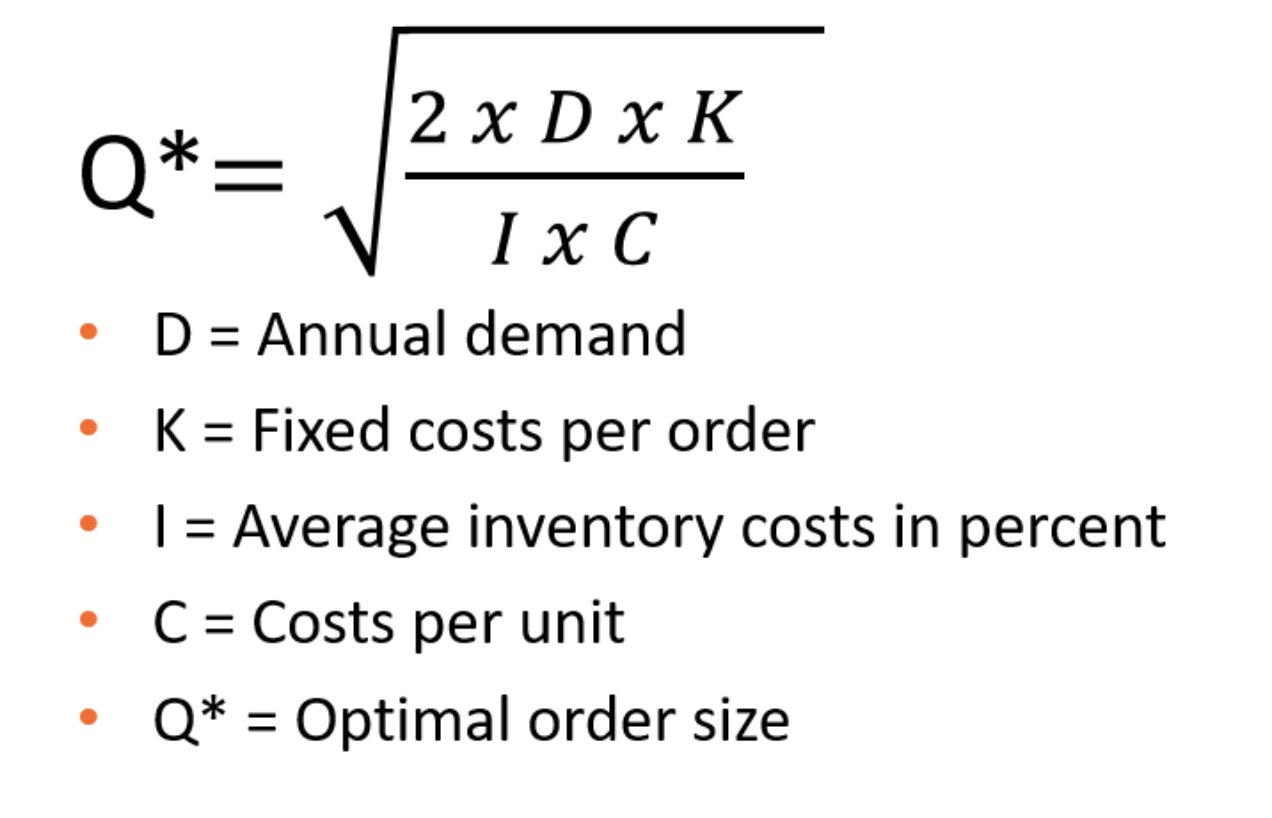
\includegraphics[width=\hsize]{figures/implementation/eoq.png}
%        \caption{EOQ formlen - Beregning af den optimale bestillingsmængde}
%        \label{fig:eoq}
%    \end{figure}
%\end{landscape}

Der kan så laves en \verb|productMap|, som lægges i \verb|PeriodicPlan| så der kan oprettes \verb|StorageOrder|s med de optimale bestillingsmængder. Desværre blev denne feature ikke implementeret færdig.

\subsection{Regression algoritme}
For at kunne forudsige salget af produkter i forskellige tidsperioder skal en algoritme, der kan leve op til kravet om, at forudsige tendenser ud fra data og heraf estimere en optimal bestillingsmængde.

Simpel matematisk regression var metoden vi valgte, eftersom det er simpelt at implementere og vi har tidligere erfaring med regression. Det er brugt til Use Cases, hvor regression giver mening at bruge. Der blev antaget at implementationen af vores egen regressions algoritme 100\% bunden ville være ekstremt tidkrævende, og beslutningen om at basere vores logik på andet kode blev truffet.

Mark Gaynor's Github repository kaldet "Multiple linear regression in Java" \cite{MarkGaynorRegressin} bruges som bunden i vores algoritme, dog har vi lavet ændringer som f.eks. at brugen af strategy pattern \cite{Larman2004}, og forsøget på at understøtte regression som kan være flere-dimensionelt. 

I \texttt{Main} ses det at der tilføjes tre features til \texttt{Observation}, heat, price og sold. Når der udføres regression over disse features, vil der blive udarbejdet en regressionsmodel med 3 dimensioner. For hver ny feature man vil måle ud fra, bliver den tilføjet som feature, og tilføjer endnu en dimension på regressionsmodellen. Dog bliver det også en tungere process hurtigt jo flere dimensioner der tilføjes. 

\section{Singleton og SQL queries}
For at kunne snakke sammen med databasen kræves der både en database forbindelse (DBConnection), samt SQL queries eller statements som kan sendes til databasen. Som vist i designklassediagrammet\ref{fig:designclassdiagram} er der brugt en interface klasse til alle SQL klasserne. Dette er en del af DAO mønstret\cite{DAO}. SQL klasserne, såsom \texttt{StoragePlanSqlStore} står for at oprette og sende \texttt{PreparedStatement} til databasen for at kommunikere med den. Sådan kan data hentes, ændres, slettes og lagres i en database. 

\subsection{PeriodicPlanSqlStore.getByStoragePlan}
Et godt eksempel på en DAO metode der bruget mange sql principper er PeriodicPlanSqlStore.getByStoragePlan \ref{lst:getByStoragePlan}, denne metode er brugt til at hente alle \texttt{PeriodicPlan} fra som en specific \texttt{StoragePlan} indeholder

Metoden starter med at sende en simpel \texttt{SELECT} query som henter rows'ne fra \texttt{periodic\_plans} hvor \texttt{storage\_plan\_id} er den givne \texttt{StoragePlan}, alle planerne bliver lagt i et map, med deres id som key, dette gøres eftersom at den følgene query finder all producterne for alle produkterne tilsvarende de her \texttt{PeriodicPlan}s

Enden af querien for \texttt{Product}s er dynamaisk generede eftersom at mængden af \texttt{PeriodicPlan}s i en \texttt{StoragePlan} ikke er fixed, for at generer enden a \texttt{WHERE} clausen laves en ny \texttt{String} array med størelsen som er lig mængden af \texttt{PeridicPlan}s som vi hentede fra første query, den array er så directe lavet om til en stream, hvor vi kalder map metoden til at lave alle entries indtil en \texttt{"periodic\_plan\_id = ?"}, de her bliver så joined sammen med \texttt{" OR "}, alt dette betyder at vi har $n$ \texttt{"periodic\_plan\_id = ?"} hvor $n$ er hvor mange \texttt{PeriodicPlan}s vi har, og mellem hver 2 af dem er der \texttt{" OR "}.

fx, hvis der var 5 \texttt{PeriodicPlan}s vil querien så sådan ud \texttt{"SELECT product\_id, amount, periodic\_plan\_id, cost, name FROM plan\_lines INNER JOIN products ON plan\_lines.product\_id = products.id WHERE periodic\_plan\_id = ? OR periodic\_plan\_id = ? OR periodic\_plan\_id = ? OR periodic\_plan\_id = ? OR periodic\_plan\_id = ?"}

Når \texttt{Product} objekterne konstrures ud fra rows'ne lægges de i directe i den korrespondent \texttt{PeriodicPlan}, hvilket kan nemt gøres pga. Map'en fra tidligerer, til sidst laves value'sne fra mappen om til en liste som bliver lags i \texttt{StoragePlan}'en fra argumentet og returneret

\begin{listing}
    \begin{minted}
    [
        frame=lines,
        framesep=2mm,
        baselinestretch=1.2,
        bgcolor=LightGray,
        fontsize=\footnotesize,
        linenos,
        breaklines
    ]{java}
@Override
public List<PeriodicPlan> getByStoragePlan(StoragePlan storagePlan) throws DataAccessException {
    try {
        PreparedStatement stmt = DBConnection.getInstance().getConnection().prepareStatement("SELECT start_period, end_period, id FROM periodic_plans WHERE storage_plan_id = ?");
        stmt.setInt(1, storagePlan.getId());
        NullableResultSet result = new NullableResultSet(stmt.executeQuery());
        Map<Integer, PeriodicPlan> plans = new HashMap<>();
        while (result.next()) {
            int id = result.getInt("id");
            plans.put(id, new PeriodicPlan(new HashMap<>(), new Period(result.getInt("start_period"), result.getInt("end_period")), null, id));
        }
        stmt = DBConnection.getInstance().getConnection().prepareStatement("SELECT product_id, amount, periodic_plan_id, cost, name FROM plan_lines INNER JOIN products ON plan_lines.product_id = products.id WHERE " + Arrays.stream(new String[plans.size()]).map(x -> "periodic_plan_id = ?").collect(Collectors.joining(" OR ")));
        int i = 1;
        for (Integer key : plans.keySet()) {
            stmt.setInt(i++, key);
        }
        result = new NullableResultSet(stmt.executeQuery());
        while (result.next()) {
            plans.get(result.getInt("periodic_plan_id")).getProductMap().put(new Product(result.getInt("cost"), result.getString("name"), null, result.getInt("product_id")), result.getInt("amount"));
        }

        List<PeriodicPlan> plansList = new ArrayList<>(plans.values());
        storagePlan.setPeriodicPlans(plansList);
        return plansList;
    } catch (SQLException e) {
        throw new DataAccessException(e.getMessage(), e);
    }
}
    \end{minted}
    \caption{PeriodicPlanSqlStore.getByStoragePlan\label{lst:getByStoragePlan}}
\end{listing}



\section{Parallelitet}\label{ch:parallelitet}
Parallelitet er processen hvorved at dele af et program, kan køres på samme tid. Dele af programmer, som køres parallelt kaldes \texttt{Threads}\cite{JavaThreads}. Threads af en abstraktion, som benyttes i high-level programmerings sprog, som f.eks Java\cite{HighLevel}. Threads er meget ofte ydeevne-optimerende, eftersom at en moderne CPU meget ofte har flere kerner, hvilket resultere i at koden fra en thread ikke er afhængig af eksekveringen af koden fra en anden thread. Dette scenarie er det dog kun relevant, hvis der eksekveres en svær algoritme. Threads er også ydeevne-optimerende når det kommer til IO, eftersom at IO operationer ofte er langsommere, ift. læsning fra RAM eller læsning fra CPU cache\cite{OperatingSystems}. Et scenerie hvor et program henter mange forskellige billeder fra internettet~\ref{lst:badParralelExample}, er i dette eksempel \texttt{fetchImage(n)} som ses på kodeeksempel \ref{lst:badParralelExample}. Den henter billedet med ID fra en remote server, hvilket ikke er optimalt, fordi metoden \texttt{fetchAllTheImages} først venter på det første kald af \texttt{fetchImage} før den starter det næste. I dette eksempel har resultatet af første \texttt{fetchImage} kald ingen effekt på det næste. Det vil sige at metoden kunne blive paralleliseret~\ref{lst:goodParralelExample} og alle \texttt{fetchImage} metoder, som bruger ~100\% af eksekveringenstiden på at vente på et IO svar, kan køre på samtidigt. I denne nye version har vi stadig det samme loop, der er dog nogle ændringer: \texttt{finalI} er lavet fordi \texttt{i} kan ændre sig før Thread'en bliver kaldt. Dette resulterer i \texttt{fetchImage} metoder, der henter de forkerte billeder. I stedet for at kalde \texttt{fetchImage} metoden, så laves en Thread, som kalder den. 
Dernest lægges den i \texttt{threads} listen, og til sidst kaldes \texttt{join} metoden på alle threads for at sikre de er færdige før \texttt{fetchAllTheImages} afsluttes.

\begin{listing}
    \begin{minted}
    [
        frame=lines,
        framesep=2mm,
        baselinestretch=1.2,
        bgcolor=LightGray,
        fontsize=\footnotesize,
        linenos
    ]{java}
public void fetchAllTheImages(int index) {
    for(int i = 0; i < index; i++) {
        fetchImage(i + 1);
    }
}
    \end{minted}
    \caption{Eksempel på ingen brug af parallelitet\label{lst:badParralelExample}}
\end{listing}

\begin{listing}
    \begin{minted}
    [
        frame=lines,
        framesep=2mm,
        baselinestretch=1.2,
        bgcolor=LightGray,
        fontsize=\footnotesize,
        linenos
    ]{java}
public void fetchAllTheImages(int index) {
    List<Thread> threads = new ArrayList<>();
    for(int i = 0; i < index; i++) {
        final int finalI = i + 1;
        Thread thread = new Thread(() -> fetchImage(finalI));
        thread.start();
        threads.add(threads);
    }
    for(Thread thread : threads){
        try {
            thread.join();
        } catch (InterruptedException ignored) {

        }
    }
}
    \end{minted}
    \caption{Eksempel på brug af parallelitet\label{lst:goodParralelExample}}
\end{listing}

Et godt eksempel på brug af parallelitet i dette projekt, kan findes i metoden \texttt{save()} i klassen 
\texttt{PeriodicPlanController}~\ref{lst:ourParralelExample}, her er alle 3 \texttt{store.update()} samt \texttt{store.delete()} langsomme IO operationer, så denne metode gør som~\ref{lst:goodParralelExample}, laver parallelitet med threads, starter dem, og til sidsts venter på de er færdige.     
 
\begin{listing}
    \begin{minted}
    [
        frame=lines,
        framesep=2mm,
        baselinestretch=1.2,
        bgcolor=LightGray,
        fontsize=\footnotesize,
        linenos
    ]{java}
    public void save() {
        Thread deleteThread = new Thread(() -> {
            try {
                store.delete(toDelete);
            } catch (DataAccessException ignored) {

            }
        });
        Thread update1Thread = new Thread(() -> {
            try {
                store.update(left, false);
            } catch (DataAccessException ignored) {

            }
        });
        Thread update2Thread = new Thread(() -> {
            try {
                store.update(current);
            } catch (DataAccessException ignored) {

            }
        });
        Thread update3Thread = new Thread(() -> {
            try {
                store.update(right, false);
            } catch (DataAccessException ignored) {

            }
        });
        deleteThread.start();
        update1Thread.start();
        update2Thread.start();
        update3Thread.start();
        try {
            deleteThread.join();
            update1Thread.join();
            update2Thread.join();
            update3Thread.join();
        } catch (InterruptedException ignored) {

        }
    }}
    \end{minted}
    \caption{Eksempel på brug af parallelitet\label{lst:ourParralelExample}}
\end{listing}

\section{UI} 
Når programmet åbnes, åbnes vinduet Lagerplaner som viser en liste over nuværende lagerplaner, og en knap "Generer ny lagerplan" som fører brugeren videre til endnu et vindue. Dette vindue er baseret på mock up figur \ref{fig:3storage} fra bilag \ref{app:mockups}. Vinduet er vist på figur \ref{fig:lagerplaner}. 

"Nuværende lagerplaner:" er tom fra starten, men som man tilføjer nye lagerplaner, kommer de oprettede lagerplaner frem på listen. Dette er til forskel fra figuren, der i stedet viser enkelte varer. Det var besluttet at være bedre med enkelte lagerplaner, sådan man derinde kunne se de forskellige produkter. 
Når der er oprettet en lagerplan på listen, kan man trykke på planen for at gå ind og redigere den. 

Knappen "Generer ny lagerplan" åbner vinduet Periodeplaner som ses på figur \ref{fig:periodeplaner}, som viser brugeren en periodeplan-liste for den genererede plan, samt et tekstfelt, hvor man kan navngive sin plan. Her er 3 handlingsknapper, "Aktiv", "Gem", og "Slet". 
"Aktiv" er speciel, fordi den har 2 stadier. Den kan være være "on" eller "off". Den er "off" fra start. Denne knap er til for at bestemme om planen er nuværende aktiv eller ikke. "Gem" knappen er ret simpel. Den gemmer alle de ændringer og tilføjelser der er lavet til den nye plan. "Slet" knappen sletter den nuværende lagerplan, som brugeren er inde at redigerere i. 
Der ses også "Periode planer for <navn>:" har en liste over udvalgte perioder. Her vælger man en bestemt periode som så åbner Periodeplan vinduet som ses på figur \ref{fig:periodeplan}. Her kan man finpudse perioden til eget behov, og tilføje eller fjerne is produkter.   

"TIlføj produkt" knappen åbner op for vinduet på figur \ref{fig:addprodukt}, hvori der er en liste over de is man kan vælge at tilføje. Derefter trykker man enten "OK" eller "Cancel". Den udvalgte is kommer frem på listen under "Produkter:". Når brugeren er færdig trykker man på "Gem" knappen, og lukker vinduet. 
"Fjern Produkt" knappen fungerer på samme måde og åbner vinduet på figur \ref{fig:fjernprodukt}. Den eneste forskel er, at der kun kan vælges blandt de produkter, der allerede er tilføjet til periodeplanen.

\begin{figure}[h]
    \centering
    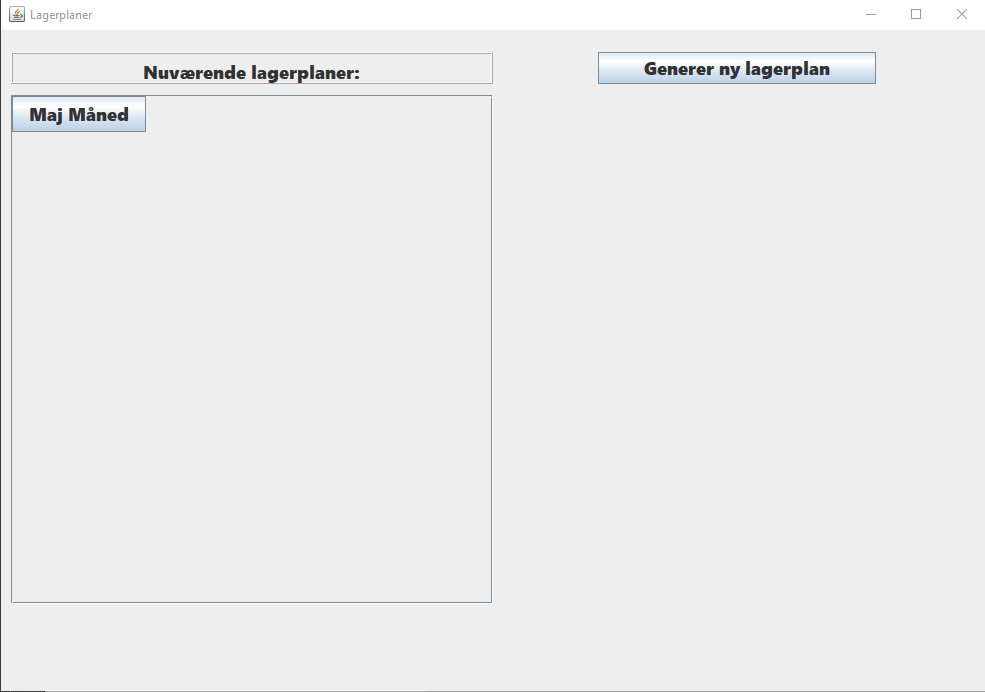
\includegraphics[width=0.7\hsize]{figures/implementation/UI/lagerplaner.png}
    \caption{Lagerplaner vinduet}
    \label{fig:lagerplaner}
\end{figure}

\begin{figure*}
    \centering
    \begin{subfigure}[b]{0.475\textwidth}
        \centering
        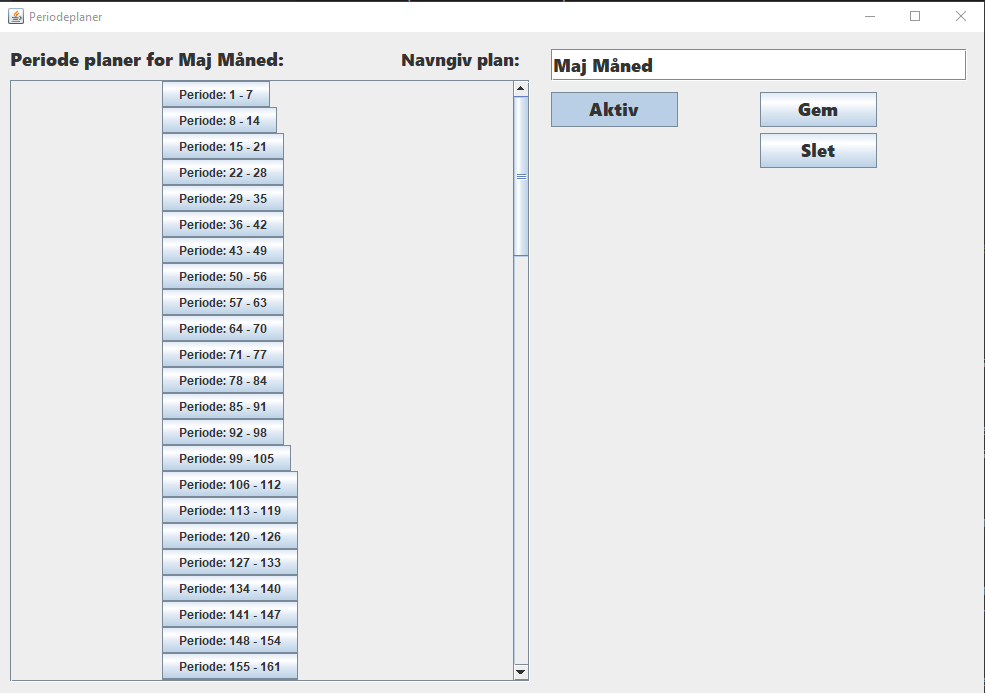
\includegraphics[width=\textwidth]{figures/implementation/UI/periodeplaner.png}
        \caption{Periodeplaner vinduet}
        \label{fig:periodeplaner}
    \end{subfigure}
    \hfill
    \begin{subfigure}[b]{0.475\textwidth}
        \centering 
        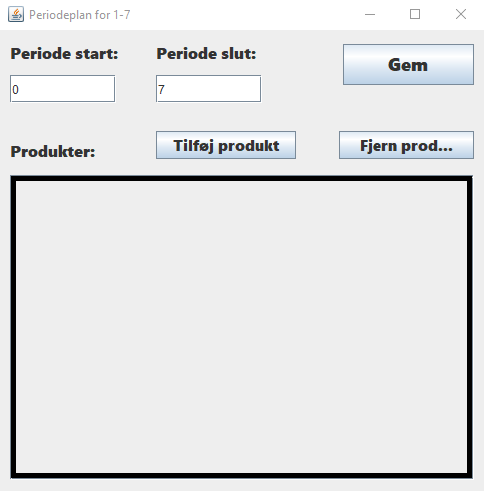
\includegraphics[width=\textwidth]{figures/implementation/UI/periodeplan.png}
        \caption{Periodeplan vinduet}
        \label{fig:periodeplan}
    \end{subfigure}
    \vskip\baselineskip
    \begin{subfigure}[b]{0.475\textwidth}
        \centering 
        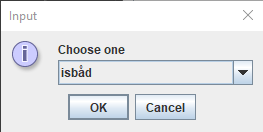
\includegraphics[width=\textwidth]{figures/implementation/UI/addprodukt.png}
        \caption{Tilføj produkt vinduet}
        \label{fig:addprodukt}
    \end{subfigure}
    \quad
    \begin{subfigure}[b]{0.475\textwidth}
        \centering 
        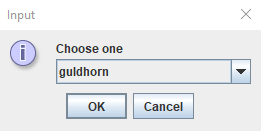
\includegraphics[width=\textwidth]{figures/implementation/UI/fjernprodukt.png}
        \caption{Fjern produkt vinduet}
        \label{fig:fjernprodukt}
    \end{subfigure}
    \caption[ GUI for automatisk lagerstyringssystem ]
    {\small GUI for automatisk lagerstyringssystem } 
    \label{fig:GUI}
\end{figure*}